\chapter{Wstęp i cel pracy. Bogna Lew, Zofia Sosińska}\label{chap:introduction}

Postrzeganie świata przed erą wielkich odkryć geograficznych znacząco różniło się od tego, które dominuje obecnie. Dawniej
decyzji strategicznych nie podejmowano na podstawie precyzyjnych map. Ludzie zmuszeni byli  budować  przestrzenny obraz
istniejącej sytuacji  w toku dyskusji z naocznymi świadkami, takimi jak dowódcy czy podróżnicy.

Współczesne gry komputerowe, których fabuła osadzona jest w tych czasach, stosuje wiele uproszczeń. Ma to na celu poprawienie jakości
rozgrywki gracza, jednakże sprawia, że nie oddaje w pełni realiów. Często obraz dzisiejszych możliwości zasłania faktyczne dowodzenie
w czasach, w których dzieje się gra. Technologia XXI wieku pozwala oficerom na wydawanie rozkazów na podstawie dokładnych map poprzez radio.
Jednak w dawniejszych czasach było to niemożliwe. Grywalna postać momentami ma wręcz boskie umiejętności i wiedzę. Zwykły człowiek nie był w
stanie w jednej chwili zobaczyć całego grywalnego świata i wydać komendę jednostkom, znajdującym się na drugim jego końcu, o przemieszczeniu
się do punktu z dokładnością do jednego metra.

“Starożytni świat widzieli inaczej, mniej płasko”\cite{gbobrektvgry}. Dobrze obrazującym ówczesne postrzeganie przestrzeni przykładem jest mapa Imperium Rzymskiego, 
pokazana na \ref{fig:mapaIR}. Czytanie jej dosłownie mija się z celem. Nie są na niej zachowane ani proporcje, ani strony świata. Mimo tego, że 
basen Morza Śródziemnego został ówcześnie dosyć dokładnie oddany, “nie wydaje się, aby Rzymianom współczesna kartograficzna wierność była potrzebna”\cite{gbobrektvgry}. 
“Dowódcy opierali się na swojej wiedzy, wiedzy wynajętych przewodników oraz informacjach zwiadowców i tubylców”\cite{gbobrektvgry}.
\begin{figure}[htbp]
    \centering
    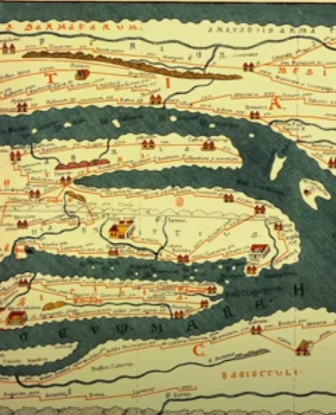
\includegraphics[width=0.5\textwidth]{images/mapaIR.png}
    \caption{Mapa basenu Morza Śródziemnego z czasów Imperium Rzymskiego}\label{fig:mapaIR}
\end{figure}

\section{Cele projektu}
Celem projektu jest zaprojektowanie oraz zaimplementowanie gry real-time strategy osadzonej we wczesnym średniowieczu i
przeznaczonej dla jednego gracza. Udostępniane przez nią mechaniki mają jak najlepiej oddawać realia tamtych czasów, przy
jednoczesnym zachowaniu podstawowych cech tego gatunku. Dodatkowo oferowane przez nią funkcjonalności nie mogą pogarszać
jakości rozgrywki.

\section{Analiza i specyfikacja wymagań}
Z punktu widzenia projektu kluczowe jest jak najdokładniejsze oddanie realiów przy jednoczesnym uwzględnieniu jakości
rozgrywki gracza oraz cech charakterystycznych dla gier typu real-time strategy. Co więcej, użytkownik będzie sterował
wybraną przez siebie postacią, wydając polecenia zaprzyjaźnionym jednostkom oraz stawiając czoła swoim przeciwnikom. Z
tego powodu kluczowe jest dobranie odpowiednich mechanik, które umożliwią osiągnięcie wymienionych założeń.

Podstawową funkcjonalnością, jaką gra musi oferować, jest sterowanie jednostkami. Gracz musi być w stanie poruszać się
wybraną przez siebie postacią oraz dowodzić swoją drużyną przy zachowaniu realiów średniowiecznej komunikacji. Dlatego
gra powinna udostępnić mechanizm przekazywania informacji zarówno pomiędzy jednostkami znajdującymi się obok siebie, jak
i znacząco od siebie oddalonymi. Konieczne będzie wprowadzenie systemu dialogów, dzięki któremu gracz będzie mógł wchodzić
w interakcję z innymi postaciami, pozyskiwać informację oraz wpływać na dynamikę świata.

Mechaniką, która ma najistotniejszy wpływ na postrzeganie świata w grze, jest sposób nawigacji. Musi ona jednocześnie
umożliwiać graczowi bez problemu zorientować się w terenie oraz nie odbiegać przy tym od realiów tamtych czasów. Z tego
powodu, niemożliwe jest wykorzystanie najpopularniejszego rozwiązania stosowanego w większości gier, jakim jest minimapa.

Kolejną mechaniką typową dla gier RTS, którą gra powinna posiadać, jest budowanie budynków. Jest to charakterystyczna
funkcjonalność, która dodatkowo urozmaica rozgrywkę. Istotną kwestią jest, aby obiekty były tworzone poprawnie oraz oddawały
realia wybranej epoki. Dzięki tej mechanice gracz będzie w stanie tworzyć bazy o znaczeniu strategicznym, które dodatkowo
pomogą mu we wzmacnianiu swoich postaci.

Dodatkowo gra musi udostępniać podstawową funkcjonalność swojego gatunku, czyli sterowanych przez sztuczną inteligencję
przeciwników. Powinni oni wykonywać ataki typowe dla realiów epoki oraz potrafić poprawnie określić swój cel. Co więcej,
powinni oni inicjować walkę z graczem, gdy go napotkają. Z tego powodu konieczne będzie utworzenie mechanizmu walki, który
obsłuży zachowanie postaci biorących w udział w starciu, jego przebieg oraz umożliwi użytkownikowi wykonywanie akcji
swoją postacią.

Konieczne będzie utworzenie interfejsu graficznego, który w czytelny sposób wyświetli graczowi aktualny stan gry, pomoże
mu w nawigacji i poznawaniu świata oraz przedstawi możliwe do podjęcia akcje. Najważniejszymi jego cechami będą prostota
i intuicyjność, aby nie przytłoczyć użytkownika ogromem i skomplikowaniem informacji. Jego celem ma być pogłębienie immersji
i przedstawienie świata z punktu widzenia granej postaci. Niezbędne będą informacje o posiadanych surowcach, czasie oraz
położeniu. Interfejs użytkownika musi też jednak dostosowywać się do sytuacji i zmieniać się tak, aby gracz miał przedstawione
możliwe opcje podczas dowodzenia walką, budowania budynków oraz prowadzenia dialogów. Kluczowe w przedstawieniu informacji
będzie stylistyczne wpasowanie się w realia gry, aby umożliwić graczowi wczucie się w epokę, w której jest osadzona fabuła.
